\subsection{Protocol and Components}
The following are the possible network architectures we will be using:
\subsubsection{ESP NOW}
ESP-NOW is a wireless communication protocol based on the data-link layer, which reduces the five layers of the OSI model to only one. This way, the data need not be transmitted through the network layer, the transport layer, the session layer, the presentation layer, and the application layer. Also, there is no need for packet headers or unpackers on each layer, which leads to a quick response reducing the delay caused by packet loss in congested networks. 
\begin{figure}[H]
    \centering
    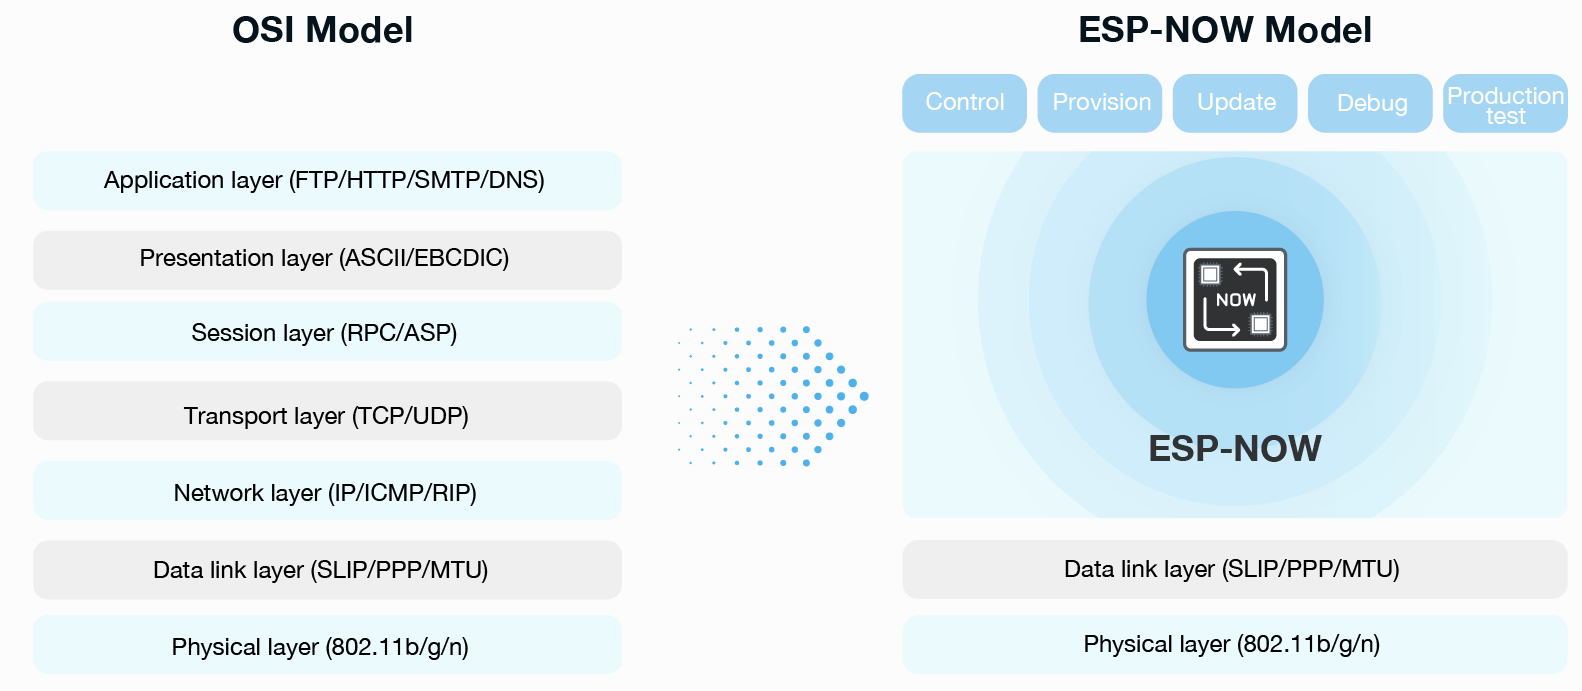
\includegraphics[width=0.75\linewidth]{Files/Images/model-en.png}
    \caption{Comparision of the OSI standard layers and the ESP NOW protocol layers}
    \label{fig:enter-label}
\end{figure}
Here are the key features of the ESP NOW Protocol:
\begin{itemize}
    \item It has a fast and user-friendly pairing method that is suitable for connecting “one-to-many” and “many-to-many” devices, while also controlling them
    \item Occupies fewer CPU and flash resources
    \item Can be used as an independent protocol that helps with device provisioning, debugging, and firmware upgrades
    \item  ECDH and AES algorithms make data transmission more secure
    \item The window synchronization mechanism greatly reduces power consumption
\end{itemize}
The devices communicates directly via the use of the data link and pairing do not require the Wi-Fi connection. Pairing can be done by initiating and multiple pairing can be done like one initiator can pair with multiple responder. Using the RSSI, during the paring the device distance can be found and that distance can be authorised and the device at that distance can be paired. The protocol supports long distance communication which will be helpful in using it outdoors. The portocol is compatible with many sensors implying its wide usability to interact among the units or the user and the unit. ESP NOW can also take data logs from multiple responders for analysis. This will facilitate the user to gather the data from the units without needing to go to the unit, again, the units can communicate the same among themselves to correctly estimate the time or find any abnormality in real time. 


\subsubsection{ESP-WIFI-MESH}
ESP-WIFI-MESH is a networking protocol that operates on top of the Wi-Fi protocol. It facilitates the interconnection of numerous devices, referred to as nodes, across a wide physical area, including both indoor and outdoor spaces, within a single WLAN (Wireless Local-Area Network).It is self-organizing and self-healing meaning the network can be built and maintained autonomously.

\begin{figure}[H]
     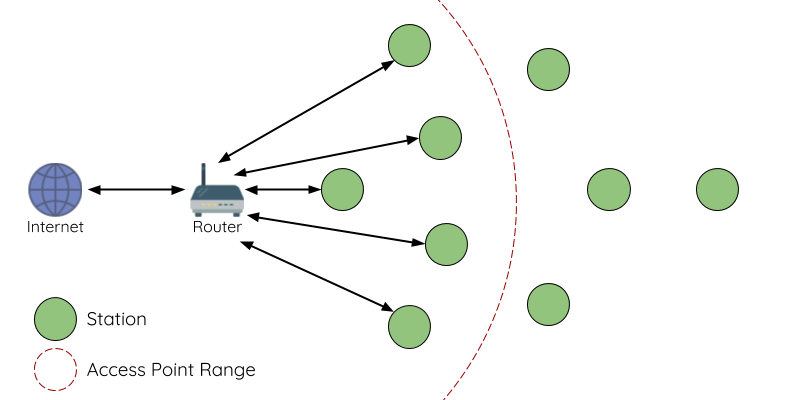
\includegraphics[width=0.5\linewidth]{Files/Images/traditional-network.png}
     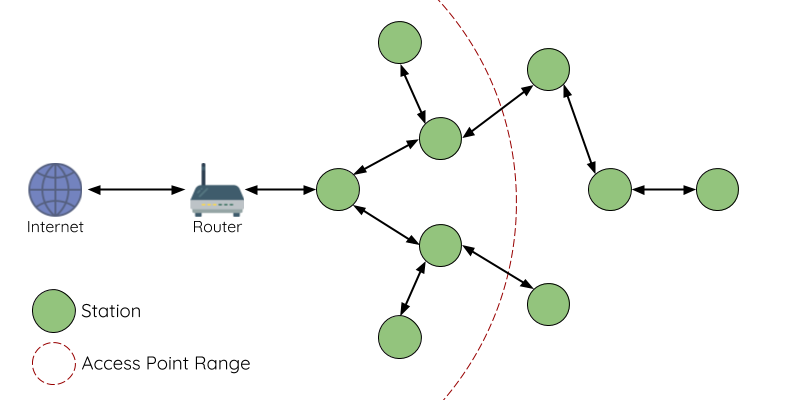
\includegraphics[width=0.55\linewidth]{Files/Images/esp-wifi-mesh.png}
     \caption{Traditional Wi-Fi Network vs ESP-WIFI-MESH Network}
     \label{fig:enter-label}

\end{figure}

Here are the key features of the ESP-WIFI-MESH:
\begin{itemize}
    \item ESP-WIFI-MESH networks do not rely on a central node like traditional infrastructure Wi-Fi networks. Instead, nodes connect with neighboring nodes, allowing for greater coverage area.
    \item Nodes within this network relay each other's transmissions, enabling interconnectivity without the need to be within range of a central node.
    \item Unlike traditional Wi-Fi networks, ESP-WIFI-MESH is not as susceptible to overloading since the number of nodes permitted on the network is not limited by a single central node's capacity.
\end{itemize}